\documentclass[a4paper]{article}

\usepackage[english]{babel}
\usepackage[utf8x]{inputenc}
\usepackage{amsmath}
\usepackage{graphicx}
\usepackage[colorinlistoftodos]{todonotes}



\title{\LARGE Avalanche \\
        \large Flexible and fast batch processing for real-time data generating applications}

\author{Authors: Michael Lin, Tongbin Wu \\
		Supervising Professor: Peter Marbach}


\begin{document}
\maketitle

\clearpage
\tableofcontents
\clearpage

\section{Introduction}
In recent years developments in cloud computing have allowed for the computation and processing of huge amounts of data.  These data sets are so large that they must be distributed over a series of computers or servers to be stored efficiently.  Hadoop was one of the first accessible forms of cloud computing, providing an infrastructure which allowed for developers to run map-reduce operations (a paradigm from functional programming) on very large distributed data sets.  More recently Twitter Storm provided an intuitive way to process streams of data by having the user create a custom logic level topography. Despite these advancements in cloud computing one scenario that remains unexplored is the execution of repetitive batch jobs on data sets, where the majority of the processed data does not change.  

This paper will outline Avalanche, a cloud infrastructure which allows for fast and scalable batch processing of information.  This infrastructure is ideal for scenarios in which a batch job is performed at regular time intervals over which the majority of the processed data does not change. Avalanche reduces overall batch computation time by leveraging the fact that the majority of the computations, necessary to produce the final output, were performed in the previous batch job because of data similarity.  Another advantage of Avalanche is it allows for the user to define a logic level topology of nodes and directed edges which governs how the computation problem is to be broken down.  At each node the data will be processed producing an output which becomes the input of the nodes connected by a directed edge.  This output data is accessible to the user, and allows for a large spectrum of data to be collected with only one pass over the data set.  The goal of Avalanche is to provide a fault tolerant and intuitive way to perform batch processing which maximizes the output of useful data and minimizes run time.   

\section{Motivation}
\subsection{Social Networks}
Social networking websites such as Facebook and Twitter generate terabytes of unstructured user data every day. The amount of data stored in such databases poses significant challenges for running analytics based on time, location and other criteria. For example, there is the need to compute historical trends of discussion topics or shared items on a regular basis. Fast computation of this data calls for the need of a batch processing system that not only is scalable but also requires minimal computation when part of the input is changed. Furthermore, the system needs to have a structured topology on the logical level that allows users to extract and save data at different stages of the computation. For example, when running analytics based on geographical location, one needs to consolidate statistics on national level, provincial level as well as municipal level.

\subsection{Financial Industry}
Financial analysts and investors often need an end of day report which summarizes historical stock market data and the influence of the transactions made the previous day (or over a set period of time). This data is crucial for financial analysts as it greatly affects risk analysis and as a result many of the investment decisions that will be made the next day.  This data may be generated in-house and contain data regarding the investments made the previous day as well as the companies current holdings.  The data could also come from an external source such as a data vendor who aggregates and normalizes market data from several data sources.  

Both instances require efficient batch processing and only have daily batch additions to the historical data being processed, making them prime use cases of Avalanche.  In addition to this, being able to define a structured topology on a logical level, allowing for the retrieval of data at the intermediate steps of computation would be very beneficial.  For example being able to compute company holding statistics, like the liquidity ratio, for the regional branch as well as the company in one computation would add huge value to the data being collected.

\section{Existing Cloud Computing Infrastructures}
The goal of this section is look at commonly used cloud computing infrastructures and identify important design criteria for Avalanche.  

\subsection{Hadoop and HDFS}
Apache Hadoop is an open-source software framework for parallel processing of large data sets on a cluster of computers. It was inspired by the MapReduce programming model and Google File System. Hadoop consists of a MapReduce engine and the Hadoop Distributed File System(HDFS).

In Hadoop's MapReduce framework, the Map() function splits the input data into small and independent chunks in parallel, while the Reduce() function performs a summary operation on the data output from the Map() function (see Figure~\ref{fig:HadoopArchitecture}). The Hadoop MapReduce engine consists of a single JobTracker and one TaskTracker per node. The JobTracker assigns tasks to the TaskTrackers, schedules them and monitor the TaskTrackers' activities. If any TaskTracker fails to communicate with the JobTracker within a fixed time interval, the JobTracker re-assigns the task to another TaskTracker. To minimize networking traffic, Hadoop runs each task on the machine or the rack of machines where the data is located. 

HDFS is designed for scalable and fault-tolerant storage of files for the Hadoop framework. Each Hadoop instance typically contains one NameNode and multiple DataNodes. The NameNode contains meta data for files in HDFS, which maps the name of each file to the machine where it is located. Typically, every Hadoop node contains a DataNode that sends read/write requests to the file system's client. HDFS is able to achieve fault-tolerance by replicating the data of each DataNode in two other nodes, one on the same machine as the DataNode and the other one on a different machine. The NameNode is responsible for monitoring the Heartbeat, a message sent to the node at frequent intervals, of all DataNodes. When a Heartbeat is not detected, the NameNode marks the corresponding DataNode as dead and forwards subsequent I/O requests to its replica. HDFS also supports write-once-read-many file access and high throughput streaming of data between applications and the file systems.

Hadoop is well-poised for scalable MapReduce algorithms that deploy to thousands of machines. It is a great framework for non-real-time processing of unstructured data because HDFS can store diverse types of large data logs. One of the drawbacks of the Hadoop infrastructure is that slow nodes will rate limit the overall process of a map-reduce.  To deal with this Hadoop will run often process the same inputs multiple times in parallel to exploit the differences in machine capabilities, taking the output which finishes first as the definitive output.  It is interesting to observe how small drawbacks in the overall design can be overcome.

\subsection{Twitter Storm}
Twitter Storm is similar to Hadoop superficially but rather than processing huge distributed sets it processes data streams.  Twitter Storm requires the user to define a network of bolts which are used to process the data streams.  The directed edges which connect the bolts are the input streams to be processed and the output streams emitted to (See Figure~\ref{fig:Storm_Topology}).  These user-defined topologies are expected to run indefinitely; as long as an input stream is present an output stream will be generated. 

One of the amazing features of Twitter Storm is that it is highly resilient and it guarantees 100\% data processing. Storm is able to achieve this by maintaining a MasterNode running Zookeeper and WorkerNodes for each bolt.  Like Hadoop, the MasterNode monitors the Heartbeat from each WorkerNode and redistributes the task if any WorkerNode is inactive. The synchronization and coordination between Master and Worker nodes is done through Zookeeper.  In addition to maintaining its heartbeat WorkerNodes also run a daemon called Supervisor which listens for work and manages worker processes.  This supervisor daemon locally manages failure by redistributing tasks and by restarting worker process in the event of a failure.  

The key features which make Twitter Storm appealing are that it performs a specific task, processing stream data, very well, it is scalable, fault tolerant, supports all languages and can be understood from a logical level very easily.  

\section{Problem Statement}
Prior to this section the gap in technology relating to batch processing as well as the industry need for such an infrastructure were outlined.  Before Avalanche can be designed, it necessary to define a high level understanding of the solution, which significantly narrows the scope of the problem without confining design possibilities.  

The goal of Avalanche is to process batch data at regular time intervals where the delta in the data is small.  To elaborate the input of Avalanche is expected to be large amounts of data (on the order of TB's) where the change in the data between each processing run is small.  A good data set might be the last 6 months of tweets from a particular user, with a daily batch job, so that the delta in the data between runs would be 1 day worth of tweets. 

Other inputs of Avalanche are the program to be executed on the data.  The goal is to allow the user to write a program without any knowledge of the hardware.  The program should require a similar level of complexity to Hadoop's MapReduce.

Similar to Hadoop, Avalanche will output, an overall final value of the entire data set processed.  For example an input program which counted the number of tweets contianing the word "Doritos" in a 6 month historical tweet data set would return the total number of tweets containing the word "Doritos" as its final value.  

In addition to this Avalanche must also allow for the output of data at intermediate steps in the computation.  As mentioned before Hadoop's MapReduce works in two stages Map, which transforms input elements to output elements, and Reduce, which combines the output of the Map function to make 1 output element.  The goal is to provide visibility in the Reduce step.  By performing the reduction step by consolidating data based on a common attribute, the output at each stage in the reduction can provide value.  This attribute must be specified by the user so that the proper data is collected.  It, however, is not enough to be able to specify which attribute the data should be grouped by (ie. time, geographic location), the user must have the flexibility to specify how the data will be reduced by defining an input logic level topology.  A more concrete example is given in the next section.

\section{Doritos Use Case}
Consider the scenario where the marketing department of Doritos has just launched an international Twitter campaign to promote their brand.  Over the next 6 months this marketing department would like to monitor the spread of their message by keeping track of the number of times the word Doritos is Tweeted.  In addition to the total number of Tweets containing the word Doritos, the marketing department would like to collect intermediate data such as the number of tweets for specific time ranges or geographic locations.  

\subsection{Dynamic Case}
Over the next 6 months Doritos would like to perform a daily batch process where the user would like to see the total number of tweets containing the word “Doritos” by time distribution.  The Doritos team expects the system to execute daily, appending that day’s tweets to the execution data set prior to running.  The Doritos team also expects the system to run autonomously, without minimal user maintenance, after the system has been setup and configured.

The user writes an input program, similar in complexity to MapReduce, which counts the number of tweets in a Twitter data set.  For each daily execution of the topology, in addition to the total number of tweets containing the word "Doritos", the user also expects a breakdown of this total.  This breakdown will be in the form of tweets per day, tweets per week, and tweets per month since beginning the batch job.  

\subsection{Static Case}
Doritos has collected a historical tweet data set spanning the last 6 months and would like to go back to re-examine the data to see which of its flavors are the most popular.  The Doritos marketing team can go back, specify the data set they collected over the past 6 months and run this new batch job.  Like the dynamic case the output of running this “static” batch job will include the total sum as well as a time-based breakdown of the statistic.   However, unlike in the dynamic case the “static” batch job will not will not be optimized for repeated execution.  

\subsection{Geographic}
The Doritos marketing team would also like to see how their marketing is affecting different geographical locations.  Like in the dynamic case, the user would like to count the number of times the number of tweets containing the word Doritos, but instead of breaking down the final value based on time, the breakdown would be based on geography.  

To achieve this in addition to the inputs of the dynamic case, the Doritos team would also define their own logical level topology as shown in Figure~\ref{fig:UseCaseTopology}.  And for each daily execution of the topology, the user would expect the number of tweets containing the word "Doritos" for the geographical locations US, France, England, Canada, NA, EU, and World as the output.  

The Doritos team would also like to be able to define similar topology for the static case.  Ideally the Doritos could define a topology for any arbitrary attribute of the basic data unit (ie. a Tweet).  

\section{Design Goals}
The following are the Design Goals of Avalanche.  These design goals outline what Avalanche hopes to achieve.  Keeping these goals in mind during the design process will ensure the correct issues are focused on.  

\subsection{User Complexity}
The usability of a system is crucial to its success.  Even if a system is the best solution, if the barrier of entry for a user is high, the system will remain unused.  A system must also have enough complexity to allow for a wide possibility of use cases.  Without this generality the system will be limited in its uses and ultimately dismissed as a comprehensive solution.  It is clear that a balance between usability and generality is crucial to the success of this system.  This concept must be consider for all aspects of the design that the user must interface with.  This includes the design of the system's API, the complexity of writing the input program and defining a topology.  

To illustrate this further consider the Doritos Sample Use Case.  If a system simplified user interaction by hard coding the geographic topology shown in Figure~\ref{fig:UseCaseTopology}, the system would be heavily handicapped, unable to perform other types of batch jobs such as those which group outputs based on time proximity.  On the other hand if the system allowed for very complex configurations such as topology graphs with cycles and input data sets with both tweets and Facebook status posts, all facets of the system would be very difficult to understand and use.  A balance is key to the success of this project.

\subsection{Scalability}

Scalability is another crucial aspect that needs to be taken into consideration when one is designing and implementing the system. Since the majority of commercially available hardware's storage capabilities do not exceed several TBs \cite{Seagate 5TB HDD}, these inputs are normally stored on multiple computers or servers. As the size of the input data grows from tens of TBs to hundreds of TBs or even several PBs, the number of machines required to store the data scales proportionally. Therefore, the ideal system should perform the aforementioned batch data processing tasks regardless of the number of storage devices. Similarly, the number of machines needed to store the output data should have minimal effect on the system's computing performance.

In our word count example of "Doritos", the historical tweets over the past weeks or months are too big to be stored on one machine. Furthermore, as the storage system might store these tweets based on attributes other than time stamp, they may be further broken down to smaller chunks and stored on a distributed set of machines. One should expect the input data batches to be located on a distributed storage system. However, it should be noted that even though the physically implementation of the system needs to be scalable, the logically representation of the system should still behave as one program.


\subsection{Guarantees Data Processing}
The system must provide a guarantee that all data inputted will be fully processed through the topology.  If data is not processed the output can no longer be considered representative of the data.  For example if in the Doritos Use Case 10\% of the data was not processed and those tweets are all from the UK, the company would be left with a false understanding of their marketing impacts in the UK.  If the user cannot be sure that the statistics gathered by the system are correct, the system has no use.  A system correct some of the time is useless.  

\subsection{Fault Tolerant}
As commercial servers may encounter malfunctions such as power outage\cite{Facebook Server Outage} and read/write failure\cite{Amazon EC2 Service Disruption}, the system needs to maintain its functionality when one or few of the underlying machines are failing to work properly. The system should either recover any in-memory data if a server is malfunctioning or re-compute that data through alternative mechanisms. This may involve backing up information of important processes on multiple machines and redirecting jobs from inactive processes to active processes. If, in the Doritos example, the tweets are stored in a cluster of servers based on location, and the servers for Canada are malfunctioning, the word count for Canada still needs to be calculated correctly in order for the statistics to be valid.


\section{Criteria and Constraints}
\subsection{Constraints}
The following constraints have been listed in order of descending priority.  These constraints are fundamental to the success of this project and must take priority when making design decisions.  

\subsubsection{Correctness}
The concept of output correctness was touched upon in the Design Goals section.  It is truly the most important constraint because without the correct output, faster computation time and memory efficiency are meaningless.  The task of this system is to output data based on the topology and input program of the user.  If the system cannot achieve this constraint it has failed to solve the initial problem.  As mentioned previously in order to ensure correctness it is also necessary for the system to guarantee that all input data is processed.  To test if a system meets this constraint the system will be compared with output of the slow naive solution which uses Hadoop to solve the outputs at each node of the topology (see section Design I: A Naive Approach).

\subsubsection{Performance}
For this system to be useful, it must demonstrate superior computation time and/or memory efficiency when compared with existing solutions.  To determine if a system meets this criteria it will be compared with the Hadoop naive solution discussed in the section Design I: A Naive Approach.  These tests will be run with large and long running loads so it is also necessary that the system be scalable and fault tolerant to ensure high performance.  For a system to be successful discernible benefits over the benchmark in the areas of memory efficiency and computation time must be observed.  If the proposed system is slower and more memory intensive than the existing solution - the system will serve no purpose.  

\subsection{Criteria}
The following criteria should be considered when making design decisions.

\subsubsection{Balance between Generality and User Complexity}
As mentioned in the Design goals section a good balance between generality and user complexity is crucial to the success of this project and as a result should be taken into consideration in all design decisions visible to the user.  

\subsubsection{Performance}
A high performing solution can be achieved through the optimization of several bottlenecks.  These bottlenecks are common to all cloud computing infrastructures and ultimately govern execution speed and resource consumption:

\begin{enumerate}
  \item \textbf{Maximizing the parallelization of computation}: The ideal solution should utilize the availability of idle servers in the clusters and distribute the tasks so that the computation can be done in as little time as possible. In a centralized system, the majority of computations has to be performed on a single machine or a small number of machines, which becomes the speed limiting step of the entire system. If tasks can be distributed to as many machines as possible, this will significantly reduce the overall computation time.
  
  \item \textbf{Maximizing processing of data on the machine the data is stored}: Typically, in a distributed computing system, each machine stores a portion of the total input and/or output data and also performs computation locally. For the data located on each machine, performing read and write operations locally is much faster than passing the data through networks \cite{Cloud Computing Disadvantage}. For this reason, the system should perform data computation locally whenever possible before aggregating that data and passing it on to other machines. 
   
  \item \textbf{Minimizing the amount of data that needs to be sent throughout the network}: Similar to the previous point, a high performing system should not rely heavily on sending data throughout the network to perform the computation, as this approach does not scale as the number of machine increases significantly\cite{Cloud Computing Network Bottleneck}. Transferring data excessively will saturate the network's bandwidth and reach a performance bottleneck.
\end{enumerate}

The aforementioned criteria are the metrics that distinguish a working solution from an optimal solution. If one constructs a distributed system that perform all computations in parallel, it is very likely that the system has to pass data around from one machine to another to keep all machines active. However, this will create extra burden on the network and limit the execution speed of the overall task. On the other hand, if we maximize the amount of data processed locally, the machine with the most time-consuming tasks will delay the completion of the overall system. The design of a high performing solution will take all three aspects into consideration and find a right balance between them that achieve a minimum execution time.
  

\section{Feature Set}
The following is the functionality and feature set that we hope to provide with Avalanche.  The features are listed in order of descending priority with Priority 1 being crucial to the success of the project and Priority 5 being a stretch goal.  The order of priority will heavily govern the order in which things are completed.  Priority 1 details the feature set necessary to provide the minimum viable product.  This system will not include much in the dimension of generality but will provide a system that will execute batch jobs according to a hard coded configuration.  As more lower priority features from are implemented, the generality of the solution will be expanded allowing the user to have greater control over aspects such as machine-job assignments and topologies. 

\subsection{Priority 1}
{\bf User provides three types of processes as a minimum requirement:} In the minimum case,  the system supports the static and dynamic cases described in the Doritos example. The user needs to provide a mechanism for the system to read and write data and to perform the necessary computations. This is achieved by allowing the user to input three types of processes: the first to read/write data from/to the file system, the second to compute the output from the input data, and the last to transmit data from one machine to another.

{\bf Input data is chronological and the system generates a level-based topology:} The system assumes that each batch of input data is characterized by time. Because user input is minimal, the logical topology is automatically generated by the system. The topology is in the form of levels, where each level aggregates computations on the basis of a day, a week, a month, etc. The granularity of these levels is hard coded by the system. For example, in the topology for the Doritos example as shown in Figure~\ref{fig:TopologyByTime}, the system first counts the total number of tweets on a daily basis, then sends the result to the next level which perform the same computation for a weekly basis. Subsequently, the tweet counts for each month and the entire 6 months period are also evaluated in the next two levels.

{\bf The available machines are all used for computation and storing output data:} The user also needs to specify a list of machine IDs available for data storage and computation. The system will distribute the processes among these machines evenly. The output of all the buckets in the topology will be written to the file system using the read/write process the user provided and a list of the file locations are returned to the user at the end of execution.

\subsection{Priority 2}
{\bf The user is able to specify the time intervals for each level in the topology:} With the addition of this feature the user will be able to specify the way computations are aggregated at each level.  For example if in the Doritos use case the time intervals (1 day, 2 days, 1 week) was specified, the first level would compute the number of tweets containing the word Doritos for each day in the data set.  These values would then be passed onto the second level where the count would be calculated for each pair of days. The next level would then compute a weekly output, generating a value for each week in the data set.  Finally the outputs of the third level would be combined to produce the total tweet count.  

{\bf The user is able to assign specific machines to different levels in the topology:} If the user knows which machines are more powerful it is beneficial to allow them to task these machines to lower levels in the topology (closer to the raw data), where the amount of data to be processed is more.  

\subsection{Priority 3}
{\bf The user is able to manually construct the topology through graphical user interface or code:} In case the user needs to conduct detailed analysis on tweets of the last month and compare it with tweets of the previous 6 months, the system needs to provide a mechanism by which the users can construct their own computation topology. The user should be able to connect the inputs and the outputs of the processes by modifying the configuration files of the system. Additionally, a nice-to-have feature is a graphical user interface that allows the user to drag the processes around in order to define the topology. Note that regardless of which method the user uses, the topology should be a directed acyclic graph (DAG), because otherwise the system may not comprehend the flow of data.

\subsection{Priority 4}
{\bf User is able to compute intermediary outputs based on attributes other than time:}  Without this feature the system is only able to compute outputs with respect to the dimension of time, ie. the number of “Doritos” containing tweets per day or week.  This feature allows for the user to compute outputs with respect to any attribute of the tweet.  For example in the Doritos case the number of tweets about “Doritos” for individual countries and continents could be computed by specifying a topology similar to one in Figure~\ref{fig:UseCaseTopology}.  This topology would result in the output of the number of tweets containing the word "Doritos" for the geographical locations US, France, England, Canada, NA, EU, and the World.  

When the topology was guaranteed to be based on time, if the input was chronological the system could easily map the data to the first level nodes.  If we allow for computation based on other attributes (such as geographic location) the system has no way of knowing which level 1 nodes should process what data.  This means that the user must provide a function which governs the mapping between the raw data and the nodes of the first level of processing.  

\subsection{Priority 5}
{\bf Multi-dimensional bucket processing:} In our previous discussions, the levels in the system’s topology can only process a single dimension of data. The data is either aggregated based on time (see Priorities 1 and 2) or based on other attributes such as location (see Priority 4). A stretch feature for the system is to allow each bucket to process data across multiple dimensions. For example, if Doritos were to calculate the number of tweets of “Doritos” at different levels of geographical locations across different time intervals, the system needs to allow each bucket to aggregate the number of tweets from the previous level into two dimensions before passing it to the next level. This feature may not be possible to implement and is thus the lowest priority.

\section{Design}
\subsection{Design I: A Naive Approach}

\subsubsection{Evaluation against Goals, Criteria, and Constraints}

\subsection{Design II: A Functional Solution}

\subsubsection{Evaluation against Goals, Criteria, and Constraints}

\subsection{Design III: An Optimal Solution}

\subsubsection{Justification}
\subsubsection{Evaluation against Goals, Criteria, and Constraints}
\subsubsection{Possible Improvements}

\clearpage

\begin{thebibliography}{9}

\bibitem{Hadoop Yahoo}
	"Apache Hadoop." {\it Hadoop Tutorial.} Yahoo, n.d. Web. 16 Sept. 2013.

\bibitem{Storm Twitter}
"Storm, Distributed and Fault-tolerant Realtime Computation." {\it Storm, Distributed and Fault-tolerant Realtime Computation.} Twitter, n.d. Web. 15 Sept. 2013.

\bibitem{Hadoop Twitter Blogs}
"A Storm Is Coming: More Details and Plans for Release." {\it Twitter Blogs.} Twitter, 4 Aug. 2011. Web. 15 Sept. 2013.

\bibitem{Amazon EMR}
"Get Started: Count Words with Amazon EMR." {\it Amazon Elastic MapReduce. Amazon}, 31 Mar. 2009. Web. 20 Sept. 2013.

\bibitem{Hadoop Orielly}
"Hadoop: What It Is, How It Works, and What It Can Do." {\it Strata. Oreilly}, 12 Jan. 2011. Web. 20 Sept. 2013. 

\bibitem{Hadoop Apache}
"Welcome to Apache Hadoop." Apache Software Foundation, 2012. Web. 17 Sept. 2013.

\bibitem{HDFS Apache}
Borthakur, Dhruba. "The Hadoop Distributed File System: Architecture and Design." The Apache Software Foundation, 2007. Web. 17 Sept. 2013.
\textless http://hadoop.apache.org/docs/r0.18.0/hdfs\_design.pdf‎ \textgreater.

\bibitem{Seagate 5TB HDD}
Lal Shimpi, Anand. "Seagate to Ship 5TB HDD in 2014 Using Shingled Magnetic Recording." RSS. Anand Tech, 9 Sept. 2013. Web. 22 Sept. 2013.
\textless http://anandtech.com/show/7290/seagate-to-ship-5tb-hdd-in-2014-using-shingled-magnetic-recording \textgreater.

\bibitem{Amazon EC2 Service Disruption}
"Summary of the Amazon EC2 and Amazon RDS Service Disruption." Summary of the Amazon EC2 and Amazon RDS Service Disruption. Amazon Web Services, 29 Apr. 2011. Web. 23 Sept. 2013. 
\textless http://aws.amazon.com/message/65648/ \textgreater.

\bibitem{Facebook Server Outage}
Johnson, Robert. "More Details on Today's Outage." More Details on Today's Outage. Facebook Inc., 23 Sept. 2010. Web. 23 Sept. 2013.
\textless https://www.facebook.com/note.php?note\_id=431441338919 \textgreater.

\bibitem{Cloud Computing Network Bottleneck}
Saran, Cliff. "Cloud Computing: How to Avoid a Network Bottleneck." Cloud Computing: How to Avoid a Network Bottleneck. ComputerWeekly, 3 May 2011. Web. 23 Sept. 2013. 
\textless http://www.computerweekly.com/news/1280095810/Cloud-computing-How-to-avoid-a-network-bottleneck \textgreater.

\bibitem{Cloud Computing Disadvantage}
Lowe, Doug. "Disadvantages of Cloud Computing for Networks." For Dummies. Wiley, Apr. 2013. Web. 23 Sept. 2013. \textless http://www.dummies.com/how-to/content/disadvantages-of-cloud-computing-for-networks.html \textgreater.


\end{thebibliography}

\clearpage

\appendix
\section{Figures}

\begin{figure}[!htbp]
\centering
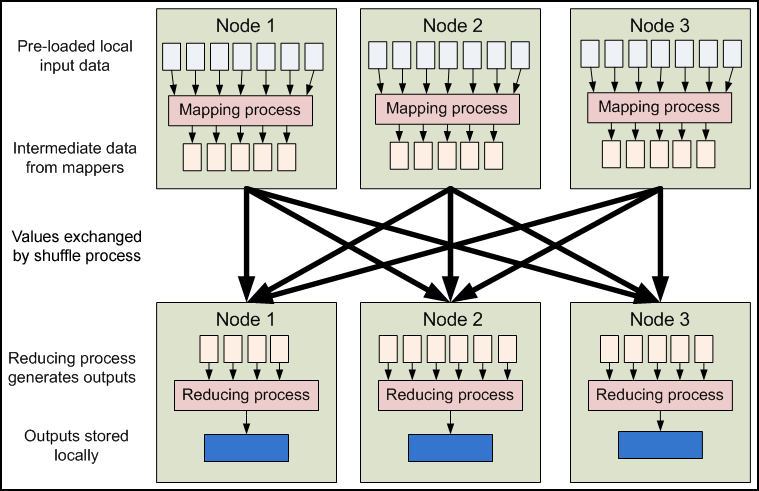
\includegraphics[width=1.0\textwidth]{images/HadoopArchitecture.png}
\caption{Hadoop Architecture}
\label{fig:HadoopArchitecture}
\end{figure}

\begin{figure}[!htbp]
\centering
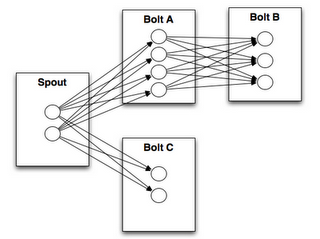
\includegraphics[width=1.0\textwidth]{images/Storm-Topology.png}
\caption{Twitter Storm Topology}
\label{fig:Storm_Topology}
\end{figure}

\begin{figure}[!htbp]
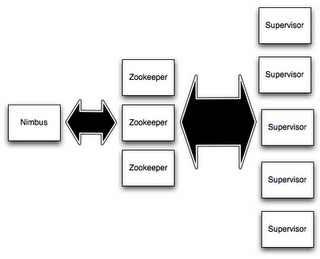
\includegraphics[width=1.0\textwidth]{images/Storm-FaultTolerance.png}
\caption{Twitter Storm Topology}
\label{fig:Storm_FaultTolerance}
\end{figure}

\begin{figure}[!htbp]
\centering
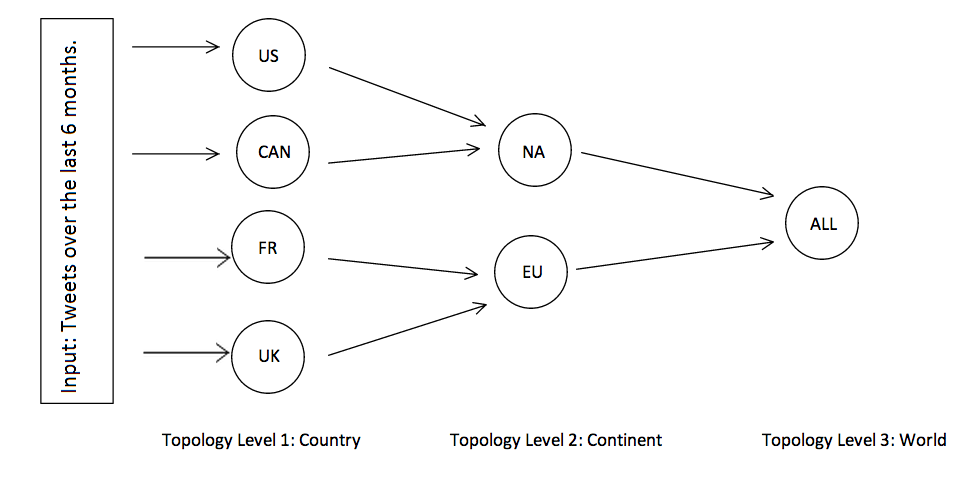
\includegraphics[width=1.0\textwidth]{images/SampleUseCaseTopology.png}
\caption{Use Case Topology (by location)}
\label{fig:UseCaseTopology}
\end{figure}

\begin{figure}[!htbp]
\centering
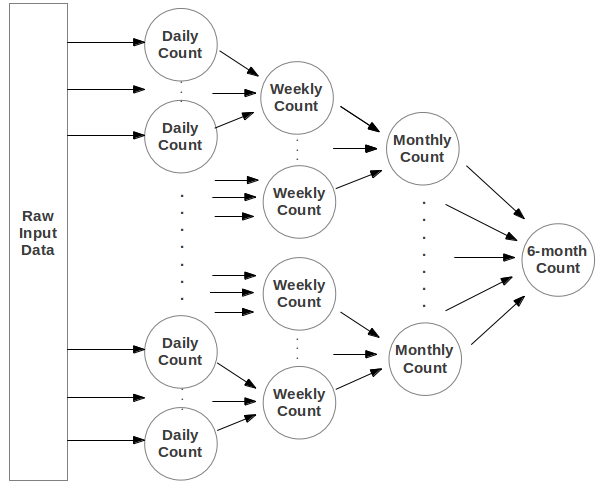
\includegraphics[width=1.0\textwidth]{images/topology_by_time.png}
\caption{Use Case Topology (by time)}
\label{fig:TopologyByTime}
\end{figure}

\end{document}
